\documentclass{article}
\usepackage{graphicx}
\usepackage[spanish]{babel}
\usepackage{float}
\usepackage{minted}
\usepackage{listings}
\usepackage{xcolor}
\usepackage{hyperref}

\lstset{
    language=bash,
    basicstyle=\ttfamily\small,  % Tipo de letra monoespaciada
    keywordstyle=\color{blue},   % Color de palabras clave
    stringstyle=\color{red},     % Color de strings
    commentstyle=\color{gray},   % Color de comentarios
    showstringspaces=false       % No mostrar espacios en strings
}

\lstdefinelanguage{SQL}{
    keywords={SELECT, FROM, WHERE, INSERT, INTO, VALUES, UPDATE, SET, DELETE, CREATE, TABLE, ALTER, DROP, INDEX},
    keywordstyle=\color{blue}\bfseries,
    morekeywords={PRIMARY, KEY, FOREIGN, NOT, NULL, AUTO_INCREMENT, DEFAULT, CONSTRAINT},
    sensitive=false,
    morestring=[b]',
    morecomment=[l]--,
    morecomment=[s]{/*}{*/},
    commentstyle=\color{gray}\ttfamily,
    stringstyle=\color{red}\ttfamily,
}

\begin{document}

% Portada
\begin{titlepage}
    \centering
    \includegraphics[width=0.4\textwidth]{logo.png} % Ajusta el nombre de la imagen según corresponda
    \\[2cm]
    {\Huge \textbf{Práctica 1: Grafana}}\\[1.5cm]
    {\Large \textit{Evaluación de Sistemas Informáticos}}\\[1cm]
    {\large 3º Grado en Informática. Mención de TI}\\[1cm]
    {\large Grupo 6}\\[1.5cm]
    \textbf{Autores:}\\[0.7cm]
    Víctor Fernández Sánchez\\
    Gonzalo Sánchez Maroto\\
    Diego Sanz Santos\\
    Rubén Verduras Cavada\\[2cm]
    \vfill
    \today
\end{titlepage}

\tableofcontents % Componer y mostar el índice
\listoffigures % Componer y mostrar el índice de tablas
\listoftables % Componer y mostrar el índice de figuras
\newpage

\section{Flask}
    Flask es un microframework escrto en Python y desarrollado para simplificar y hacer más fácil la creación de aplicaciones web bajo el patrón modelo vista controlador (MVC). Las pricipales ventajas de usar Flask son:
        \begin{itemize}
            \item Microframework: perfecto si se quiere desarrollar una app básica de manera rápida y ágil, ya que no se necesitarán muchas extensiones, y con Flask es suficiente.
            \item Incluye un servidor web de desarrollo: no se necesita una infraestructura con un servidor web para testear las aplicaciones, simplemente se puede ejecutar en un servidor web de manera sencilla.
            \item Tiene un depurador y soporte integrado para pruebas unitarias: para comprobar errores en el desarrollo.
            \item Compatibilidad con WSGI: que es un protocolo que conecta internamente el servidor web con la aplicación.
            \item Compatibilidad con Python3.
            \item Buen manejo de rutas: se deben de recibir y manipular correctamente las peticiones de los clientes y determinar a qué ruta está accediendo el cliente para ejecutar el código correcto.
            \item Soporta de manera nativa el uso de cookies.
            \item Sin ORMs: que es una técnica que permite relacionar objetos y los datos que representan.
            \item Se pueden usar sesiones.
            \item Muy óptima para construir servicios web o aplicaciones de contenido estático.
            \item Documentación formada por lista de correos y códigos en GitHub.
            \item Open Source.
        \end{itemize}

    \subsection{Python}
        Para utilizar Flask, es necesario tener instalado Python. Para ello se ejecuta el comando \lstinline{python --version}, y debe aparecer una versión de Python 3 o superior.\\
        En caso de no tener instalado Python, se puede descargar desde la página oficial de Python.

    \subsection{Entorno virtual}
        Un entorno virtual (venv) es una carpeta que contiene una instalación independiente de Python y sus dependencias, es decir, es un lugar seguro donde se pueden instalar dependencias específicas sin afectar al sistema operativo ni a otros proyectos. Sus ventajas son:
            \begin{itemize}
                \item Aislamiento: evita conflictos de versiones entre diferentes proyectos.
                \item Control: puede tener un archivo con todas las versiones usadas.
                \item Seguridad: no se modifica la instalación de Python del sistema.
                \item Portabilidad: puedes compartir tu proyecto fácilmente.
            \end{itemize}
        Para crear el entorno virtual ejecutamos el comando \lstinline{python3 -m venv env_pruebas}, para activarlo \lstinline{source env_pruebas/bin/activate}, y para desactivarlo \lstinline{deactivate}. 
        Con el entorno virtual activado, habría que instalar el paquete de Flask con el comando \lstinline{pip install flask}, y comprobarlo con \lstinline{pip show flask}.

    \subsection{Estructura de carpetas}
        Para mantener un código limpio, modular y escalable, se ha utilizado una estructura específica de carpetas con las siguientes funcionalidades:
            \begin{itemize}
                \item db: utilizada para la gestión de la base de datos.
                \item models: utilizada para definir las clases que representan las tablas de la base de datos.
                \item routes: utilizada para definir las rutas (endpoints) de la aplicación.
                \item schemas: utilizada para la validación y serialización de datos con la API.
                \item static: utilizada para almacenar archivos estáticos que el navegador debe cargar directamente.
                \item templates: utilizada para almacenar las plantillas HTML.
                \item utils: utilizada para almacenar funciones o clases auxiliares que se reutilizan en diferentes partes de la app.
            \end{itemize}

\section{Página web}
    La página web que se va a crear para esta parte de la página será una tienda online de platos de comida, en donde los usuarios podrán consultar y realizar pedidos a través de su cuenta. Las principales funcionalidades de la página web son:
        \begin{itemize}
            \item Los usuarios deben de ser capaces de registrarse e identificarse en la web.
            \item Los usuarios deben de ser capaces de consultar una descripción del producto que se vende y un menú de acceso a las distintas vistas desde una página principal.
            \item Los usuarios deben de ser capaces de consultar una lista de productos que se venden, y ser capaces de añadirlos a su carrito de la compra.
            \item Los usuarios deben de ser capaces de consultar los productos que tienen en su carrito de la compra y realizar un pedido de todos ellos.
            \item Los usuarios deben de ser capaces de consultar con más detalle cada uno de los productos.
            \item Los usuarios deben de ser capaces de consultar un historial de todos los pedidos realizados y sus detalles.
        \end{itemize}
    En base a las especificaciones de la web anteriores se han detectado una serie de vistas que debe de tener la página web, y son las siguientes:
    \begin{itemize}
        \item Página principal: en esta vista, se presenta el propósito de la web y da la posibilidad de navegar por toda ella.
        \item Registro de usuario: en esta vista, el usuario será capaz de registrarse como un usuario nuevo.
        \item Identificación de usuario: en esta vista, el usuario será capaz de identificarse en la web, si ya tiene cuenta creada.
        \item Lista de productos disponibles: en esta vista, se muestran la lista de productos que están disponibles para su venta.
        \item Detalle del producto: en esta vista, se muestra con más detalle el producto, como la información nutricional.
        \item Carrito de la compra: en esta vista, se muestra el contenido del pedido actual.
        \item Historial de pedidos:en esta vista, se muestra una lista de pedidos realizados en el pasado.
        \item Detalles de un pedido: en esta vista, se muestra en más detalle el pedido realizado, como los productos y el precio.
    \end{itemize}

    \subsection{Modelo de dominio}
        \begin{figure}[H]
            \centering
            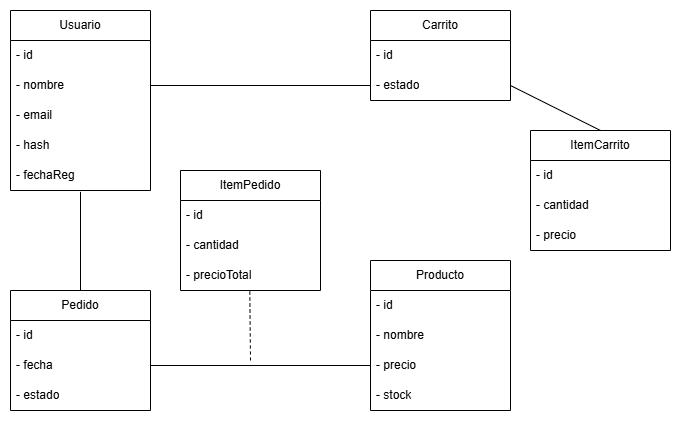
\includegraphics[width=1\linewidth]{modelo_dominio.drawio.png}
            \caption{Modelado de dominio}
            \label{fig:dom-mod}
        \end{figure}
        
    \subsection{Mapa del sitio web}
        \begin{figure}[H]
            \centering
            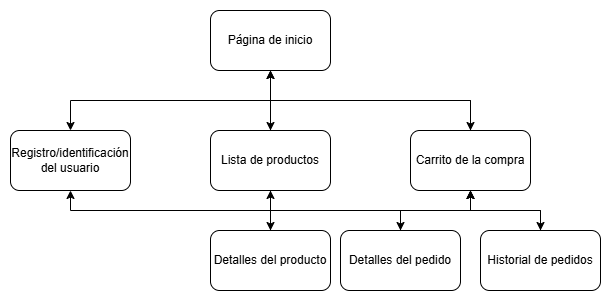
\includegraphics[width=1\linewidth]{mapa_sitio_web.drawio.png}
            \caption{Mapa del sitio web}
            \label{fig:web-map}
        \end{figure}

\end{document}
